\documentclass[a4paper, oneside]{memoir}
\usepackage[danish]{babel} % load typographical rules for the english language
\usepackage{graphics} % for \scalebox
\usepackage{hyperref} % for \href
\usepackage{xcolor} % for text color
\usepackage{enumitem} % for ordered and unordered list
\usepackage{graphicx} % for images
\usepackage{pdfpages} % for including pdfs
\usepackage{footnote} % for footnotes
\usepackage{longtable} % for tabular environment that spans multiple pages and supports footnotes
\usepackage{colortbl} % for cell coloring
\usepackage{multirow} % for \multicolumn

% https://github.com/latex3/babel/issues/51
\makeatletter\AtBeginDocument{\let\@elt\relax}\makeatother

% styling
\setsecnumdepth{subsubsection} % how deep to number sections
\setlength{\parindent}{0em} % horizontal indent for first line of paragraph
\setlength{\parskip}{1em} % vertical space between paragraphs

\newcommand{\textdesc}[1]{\textit{\textbf{#1}}}
\newcommand{\descitem}[1]{\item \textdesc{#1}}

\title{\documenttitle\\\scalebox{0.85}{\documentsubtitle}}
\author{Aslak Johansen \href{mailto:asjo@mmmi.sdu.dk}{asjo@mmmi.sdu.dk}\\Aisha Umair \href{mailto:aiu@mmmi.sdu.dk}{aiu@mmmi.sdu.dk}}

\begin{document}

\maketitle
\setcounter{tocdepth}{2}
\tableofcontentswrapper


%%%%%%%%%%%%%%%%%%%%%%%%%%%%%%%%%%%%%%%%%%%%%%%%%%%%%%%%%%%%%%%%%%%%%%%%%%%%%%%%
%%%%%%%%%%%%%%%%%%%%%%%%%%%%%%%%%%%%%%%%%%%%%%%%%%%%%%%%%%%%%%%%%%%%%%%%%%% Tema
\chapter{Semesterprojektet}

Semesterprojektet handler om programudvikling. Projektet er problemorienteret og programudviklingen er objektorienteret.

Projektarbejdet styres af en problemstilling, som projektgrupperne selv vælger og formulerer indenfor de rammer, der udstikkes på semestret.

I objektorienteret programudvikling arbejdes der med at finde en løsning på et problem gennem objektorienteret analyse- og design og at implementere denne løsning i et objektorienteret programmeringssprog.

Projektet bygger på online kurset \textbf{“Problemorienteret projektarbejde på ingeniøruddannelserne”} og kurset “Objektorienteret programmering”, som I gennemfører parallelt med projektet.  

%%%%%%%%%%%%%%%%%%%%%%%%%%%%%%%%%%%%%%%%%%%%%%%%%%%%%%%%%%%%%%%%%%%%%%%%%%%%%%%%
%%%%%%%%%%%%%%%%%%%%%%%%%%%%%%%%%%%%%%%%%%%%%%%%%%%%%%%%%%%%%%%%%%%%%%%% Projektets rammer
\section{Projektets Rammer}

Projektet er et frit projekt med følgende begrænsninger: 
\begin{enumerate}
  \item Problemstillingen skal findes inden for Vores verdensmål.
  \item Løsningen skal bygge på World of Zuul.
\end{enumerate}

Projektet skal desuden overholde de specifikke krav fra afsnit ~\ref{sec:krav}.

%%%%%%%%%%%%%%%%%%%%%%%%%%%%%%%%%%%%%%%%%%%%%%%%%%%%%%%%%%%%%%%%%%%%%%%%%%%%%%%%
%%%%%%%%%%%%%%%%%%%%%%%%%%%%%%%%%%%%%%%%%%%%%%%%%%%%%%%%%%%%%%%%%%%%%%%% Vores verdensmål

\subsection{Vores Verdensmål}
\label{sec:verdenmål}

Bestyrelsen for SDU godkendte den 17. juni 2019, at FN’s 17 verdensmål\footnote{\url{https://www.verdensmaalene.dk/maal}} fremover bliver SDU’s kompas for universitetets virke. Under overskriften ”vores verdensmål”\footnote{\url{https://www.sdu.dk/da/voresverdensmaal/verdensmaaleneogbaredygtighedpaasdu}} kommer SDU derfor til at arbejde målrettet og dedikeret med verdensmålene i hele organisationen.

I skal i projektet udvikle et softwareprogram, som bidrager til at opnå et eller flere af verdensmålene. Jeres softwareprogram skal altså være en løsning, der bidrager til at afhjælpe et af de problemer som  verdensmålene handler om.

%%%%%%%%%%%%%%%%%%%%%%%%%%%%%%%%%%%%%%%%%%%%%%%%%%%%%%%%%%%%%%%%%%%%%%%%%%%%%%%%
%%%%%%%%%%%%%%%%%%%%%%%%%%%%%%%%%%%%%%%%%%%%%%%%%%%%%%%%%%%%%%%%%%%%%%%% World of zuul

\subsection{World of Zuul}

World of Zuul er et spil udviklet af Michael Kölling og David J. Barnes. World of Zuul er modelleret efter eventyrspillet “Colossal Cave Adventure”\footnote{\url{https://en.wikipedia.org/wiki/Colossal_Cave_Adventure)}}, som blev udviklet i de tidlige 70’ere af Will Crowter og Don Woods. Cave adventure var et storslået spil, der indeholdt den utroligste underjordiske  verden af huler, gange og skakter fyldt med vidunderlige skatte, dværge og masser af magi. World of Zuul er omvendt et fuldstændigt simpelt spil helt fri for magi. Spillet indeholder rum og spil-kommandoer og det giver som udgangspunkt blot en spiller mulighed for at bevæge sig rundt i 5 rum og give tekstbaserede kommandoer.  World of zuul  venter altså blot på jeres gode ideer og på at blive udviklet!

Projektgrupperne får udleveret kildekode til spillet  og skal  videreudvikle “World of Zuul” på basis af det udleverede og deres egen problemformulering og ide til løsning.

%%%%%%%%%%%%%%%%%%%%%%%%%%%%%%%%%%%%%%%%%%%%%%%%%%%%%%%%%%%%%%%%%%%%%%%%%%%%%%%%
%%%%%%%%%%%%%%%%%%%%%%%%%%%%%%%%%%%%%%%%%%%%%%%%%%%%%%%%%%%%%%%%%%%%%%%% Inspiration

\section{Inspiration}

%%%%%%%%%%%%%%%%%%%%%%%%%%%%%%%%%%%%%%%%%%%%%%%%%%%%%%%%%%%%%%%%%%%%%%%%%%%%%%%%
%%%%%%%%%%%%%%%%%%%%%%%%%%%%%%%%%%%%%%%%%%%%%%%%%%%%%%%%%%%%%%%%%%%%%%%% Problemstillinger

\subsection{Problemstillinger}

Eksempler på problemstillinger, som jeres projekt kunne handle om: 
\begin{itemize}
  \item \textbf{Bæredygtig forvaltning og anvendelse af vand-ressourcer i Sydafrika}
    Sydafrika står over for voksende krav om at håndtere miljømæssige, sociale og økonomiske udfordringer på en holistisk og bæredygtig måde. En af de vigtigste udfordringer er bæredygtig forvaltning og anvendelse af vandressourcer. I en tid med stigende vandknaphed og pres og efterspørgsel efter vand fra alle dele af samfundet vil vand være en vigtig ressource for udvikling og for at løfte de mest marginaliserede grupper ud af fattigdom.
  \item \textbf{Reduktion af belastning af natur og begrænsning af dyre råmaterialer}
    Vi forbruger elektronik som aldrig før, og elektronik er en af verdens hurtigst voksende affaldsfraktioner. På verdensplan smider vi ifølge FN lige knap 50 millioner tons elektronik ud om året. Og kurven bliver bare ved med at stige. Hvert år smider vi store mængder af elektroniske apparater ud (husholdningsmaskiner, fladskærme, computere, batterier, biler etc.). En stor del af disse apparater eller deres bestanddele kan nemt genbruges. Dermed kan vi mindske belastningen af naturen og begrænse forbruget af dyre råmaterialer.
\end{itemize}

%%%%%%%%%%%%%%%%%%%%%%%%%%%%%%%%%%%%%%%%%%%%%%%%%%%%%%%%%%%%%%%%%%%%%%%%%%%%%%%%
%%%%%%%%%%%%%%%%%%%%%%%%%%%%%%%%%%%%%%%%%%%%%%%%%%%%%%%%%%%%%%%%%%%%%%%% Løsninger 

\subsection{Løsninger}

Jeres ideer til løsninger kan gå i flere retninger: Læringsspil, gamification eller noget helt tredje. Den grundlæggende løsningsstruktur skal blot være en person eller noget der bevæger sig gennem forskellige lokationer vha. kommandoer. 

%%%%%%%%%%%%%%%%%%%%%%%%%%%%%%%%%%%%%%%%%%%%%%%%%%%%%%%%%%%%%%%%%%%%%%%%%%%%%%%%
%%%%%%%%%%%%%%%%%%%%%%%%%%%%%%%%%%%%%%%%%%%%%%%%%%%%%%%%%%%%%%%%%%%%%%%% Inspirationskassen 

\subsection{Inspirationskassen}

Se mere i inspirationskassen (afsnit \ref{sec:inspiration}).

%%%%%%%%%%%%%%%%%%%%%%%%%%%%%%%%%%%%%%%%%%%%%%%%%%%%%%%%%%%%%%%%%%%%%%%%%%%%%%%%
%%%%%%%%%%%%%%%%%%%%%%%%%%%%%%%%%%%%%%%%%%%%%%%%%%%%%%%%%%%%%%%%%%%%%%%% Projektfaser

\section{Projektfaser}

Projektet forløber gennem hele semestret fra start til slut. Projektet inddeles i fem hovedfaser: “Projektstart”, “Problemanalyse”, “Gennemførsel”, “Færdiggørelse” og “Evaluering og refleksion”. Faserne er vist i figur \ref{fig:faser}:

\begin{figure}[tbp]
\begin{center}
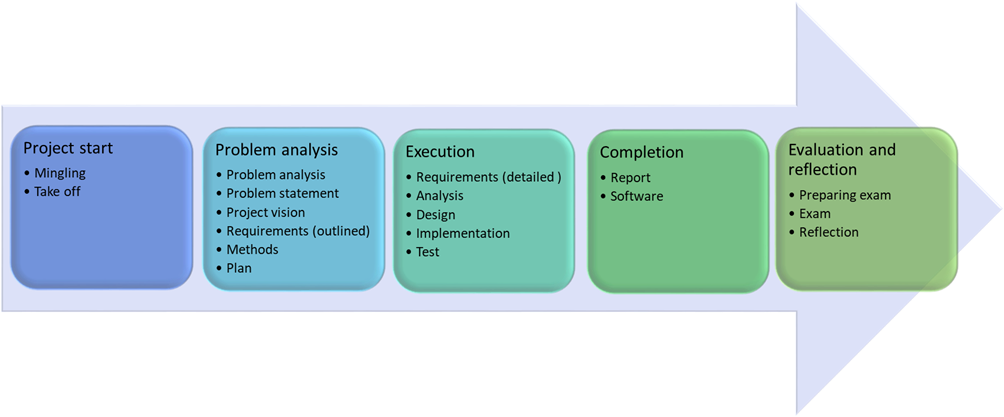
\includegraphics[width=10cm]{images/faser.png}
\caption{Projekt Faser}\label{fig:faser}
\end{center}
\end{figure}

Det nærmere indhold af faserne fremgår af assignments på itslearning.

De tidsmæssige rammer for projektet sættes af semesterplanen.

%%%%%%%%%%%%%%%%%%%%%%%%%%%%%%%%%%%%%%%%%%%%%%%%%%%%%%%%%%%%%%%%%%%%%%%%%%%%%%%%
%%%%%%%%%%%%%%%%%%%%%%%%%%%%%%%%%%%%%%%%%%%%%%%%%%%%%%%%%%%%%%%%%%%%%%%% Arbejdet og samarbejdet 

\section{Arbejdet og Samarbejdet}

Projektets omfang er 10 ECTS point. Det svarer til 1/3 af den samlede indsats på et semester, eller til at I hver for sig har en arbejdsindsats på 250-300 timer på projektet. Tirsdag er fast projektdag, hvor gruppen har en projektarbejdsplads til rådighed hele dagen. Projektgruppen kan udover den faste dag selv planlægge andre tidspunkter til projektarbejdet.

I projektgruppen laver I tidligt i projektforløbet en \textbf{samarbejdsaftale}, der beskriver hvordan arbejdet og samarbejdet skal foregå.  

Der skrives \textbf{gruppelogbog} gennem hele projektforløbet. Gruppelogbog indeholder dagsordener og mødereferater af alle møder, herunder interne møder, arrangementer på tværs af projektgrupper og vejledningsmøder. 


%%%%%%%%%%%%%%%%%%%%%%%%%%%%%%%%%%%%%%%%%%%%%%%%%%%%%%%%%%%%%%%%%%%%%%%%%%%%%%%%
%%%%%%%%%%%%%%%%%%%%%%%%%%%%%%%%%%%%%%%%%%%%%%%%%%%%%%%%%%%%%%%%%%%%%%%% Projektvejledning

\section{Projektvejledning}

Hver projektgruppe har en projektvejleder. Vejledningen foregår på vejledningsmøder og ved arrangementer på tværs af projektgrupper. Vejledningsmøder og arrangementer foregår på den faste projektdag. 
Projektgruppen laver tidligt i projektforløbet en vejlederaftale, der beskriver form og indhold af vejledningen, møder, skriftlige oplæg og tidsplan for projektet.


%%%%%%%%%%%%%%%%%%%%%%%%%%%%%%%%%%%%%%%%%%%%%%%%%%%%%%%%%%%%%%%%%%%%%%%%%%%%%%%%
%%%%%%%%%%%%%%%%%%%%%%%%%%%%%%%%%%%%%%%%%%%%%%%%%%%%%%%%%%%%%%%%%%%%%%%% Projektværktøjer 
\section{Projektværktøjer}

%%%%%%%%%%%%%%%%%%%%%%%%%%%%%%%%%%%%%%%%%%%%%%%%%%%%%%%%%%%%%%%%%%%%%%%%%%%%%%%%
%%%%%%%%%%%%%%%%%%%%%%%%%%%%%%%%%%%%%%%%%%%%%%%%%%%%%%%%%%%%%%%%%%%%%%%% IDE

\subsection{IDE}

IDE eller “Integrated Development Environment” er det værktøj som anvendes til at arbejde med udvikling af software i projektet herunder kodeskrivning, samt fejlfinding og test af programkode. Der undervises i oprettelse af kodeprojekter og gennemgang af forskellige kodeprojekttyper, anvendelse af kodeeditoren, afvikling af kode, fejlfinding og test i forbindelse med programmeringsundervisningen.

%%%%%%%%%%%%%%%%%%%%%%%%%%%%%%%%%%%%%%%%%%%%%%%%%%%%%%%%%%%%%%%%%%%%%%%%%%%%%%%%
%%%%%%%%%%%%%%%%%%%%%%%%%%%%%%%%%%%%%%%%%%%%%%%%%%%%%%%%%%%%%%%%%%%%%%%% GitHub  

\subsection{GitHub}

GitHub bruges til \textbf{opbevaring af kode på et udviklingsprojekt}. GitHub giver mulighed for versionsstyring af koden og støtter samarbejde.

Github bruges også til  \textbf{gruppelogbog} (wiki) og til at give overblik over gruppemedlemmernes indsats (insights).

Der introduceres til GitHub logskrivning i begyndelsen af semestret og der undervises i GitHub forbindelse med programmeringsundervisningen.

%%%%%%%%%%%%%%%%%%%%%%%%%%%%%%%%%%%%%%%%%%%%%%%%%%%%%%%%%%%%%%%%%%%%%%%%%%%%%%%%
%%%%%%%%%%%%%%%%%%%%%%%%%%%%%%%%%%%%%%%%%%%%%%%%%%%%%%%%%%%%%%%%%%%%%%%% Formidlingsværktøjer  

\subsection{Formidlingsværktøjer}

Der er ingen krav til hvad der bruges til formidling af projektet, men der er flere gode muligheder.

Som studerende ved SDU har du mulighed for at få Microsoft Office uden beregning.  Universitetet stiller Office 365 gratis til rådighed.  Office 365 kan bruges til udarbejdelse af dokumenter og præsentationer, herunder posters. I Office 365 kan du dele dokumenter med andre og samarbejde om skrivning af dokumenter med andre. 

Alternativer til Office 365: Google “office” (docs, sheet, drive) og \LaTeX. \LaTeX har en læringskurve, men erfaring med dette system vil give pote når I kommer til uddannelsens afsluttende opgave.

%%%%%%%%%%%%%%%%%%%%%%%%%%%%%%%%%%%%%%%%%%%%%%%%%%%%%%%%%%%%%%%%%%%%%%%%%%%%%%%%
%%%%%%%%%%%%%%%%%%%%%%%%%%%%%%%%%%%%%%%%%%%%%%%%%%%%%%%%%%%%%%%%%%%%%%%% Specifikke krav

\section{Appendiks 1: Specifikke Krav}\label{sec:krav}

%%%%%%%%%%%%%%%%%%%%%%%%%%%%%%%%%%%%%%%%%%%%%%%%%%%%%%%%%%%%%%%%%%%%%%%%%%%%%%%%
%%%%%%%%%%%%%%%%%%%%%%%%%%%%%%%%%%%%%%%%%%%%%%%%%%%%%%%%%%%%%%%%%%%%%%%% Specifikke krav til projektet

\subsection{Specifikke krav til projektet}

\begin{itemize}
  \item Projektet skal bygges op omkring den udleverede kildekode til spillet ”The World of Zuul”. \\
  Spillet i den udleverede kildekode er meget simpelt. Den implementerede funktionalitet giver udelukkende mulighed for at give et tekstbaseret input, hvor man som spiller har mulighed for at bevæge sig rundt i 5 rum. 
  \item Den udleverede kildekode skal udforskes som en del af problemanalysen. Udforskningen skal indgå i projektgrundlaget.
  \item Den udleverede kildekode skal udvides i løbet af gennemførselsfasen. \\
    Kildekoden skal som minimum udvides med 
    \begin{itemize}
      \item Flere rum/lokationer
      \item Bevægelse mellem rummene
      \item Genstande i rummene 
      \item Flere kommandoer
      \item Funktionalitet afhængig af problemformulering
      \item Tekstbaseret brugergrænseflade (delforløb 1)
      \item Grafisk brugergrænseflade (delforløb 2)
      \item Lagdeling af klasser, samt 
      \item Elementer efter eget valg
    \end{itemize}
  \item Deling af kode
    \begin{itemize}
      \item Alle i gruppen skal have adgang til gruppens kode og I skal kunne styre forskellige udgaver (versioner) af de forskellige klasser. I skal bruge GitHub til deling af koden og som versionsstyringsværktøj.
    \end{itemize}
\end{itemize}

%%%%%%%%%%%%%%%%%%%%%%%%%%%%%%%%%%%%%%%%%%%%%%%%%%%%%%%%%%%%%%%%%%%%%%%%%%%%%%%%
%%%%%%%%%%%%%%%%%%%%%%%%%%%%%%%%%%%%%%%%%%%%%%%%%%%%%%%%%%%%%%%%%%%%%%%% Ideer til udvidelse af det grundlæggende spil

\subsection{Ideer til Udvidelse af det Grundlæggende Spil}

Ideer som I kan overveje:
\begin{itemize}
  \item at have genstande der kan samles op, og  andre der ikke kan, og om der skal være en begrænset kapacitet hos brugeren mht. hvor mange genstande, der samtidig kan være opsamlet.
  \item at have et resultat der kan opnås og en situation der fortæller at resultatet er nået. Vinde, og eventuelt tabe. Bestå, eller ikke bestå. Eller \ldots
  \item at have flere karakterer (person, monstre, guide, læge, eller lignende), der kan bevæge sig imellem rummene, og som brugeren kan interagere med.
  \item at have et pointsystem, så man får point efter hvor godt man har klaret sig og hvor langt man er nået.
\end{itemize}

%%%%%%%%%%%%%%%%%%%%%%%%%%%%%%%%%%%%%%%%%%%%%%%%%%%%%%%%%%%%%%%%%%%%%%%%%%%%%%%%
%%%%%%%%%%%%%%%%%%%%%%%%%%%%%%%%%%%%%%%%%%%%%%%%%%%%%%%%%%%%%%%%%%%%%%%% Krav til projektforløbet

\subsection{Krav til Projektforløbet}

Semesterplanen skal overholdes.

Gennemførelsesfasen skal have to delforløb, som projektgrupperne planlægger det nærmere indhold af. Der bør være følgende fokus i de to delforløb:

\begin{enumerate}
  \item Delforløb 1 - grundlæggende udvidelse af den udleverede kildekode
    \begin{enumerate}
      \item Flere rum/lokationer
      \item Bevægelse mellem rummene
      \item Genstande i rummene 
      \item Flere kommandoer
      \item Grundlæggende funktionalitet afhængig af problemformulering
      \item Tekstbaseret brugergrænseflade
      \item Elementer efter eget valg
    \end{enumerate}
  \item Delforløb 2 - Udvidelse og forfining af resultatet fra første delforløb
    \begin{enumerate}
      \item Mere funktionalitet 
      \item Grafisk brugergrænseflade
      \item Lagdeling af klasser
      \item Elementer efter eget valg
    \end{enumerate}
\end{enumerate}

%%%%%%%%%%%%%%%%%%%%%%%%%%%%%%%%%%%%%%%%%%%%%%%%%%%%%%%%%%%%%%%%%%%%%%%%%%%%%%%%
%%%%%%%%%%%%%%%%%%%%%%%%%%%%%%%%%%%%%%%%%%%%%%%%%%%%%%%%%%%%%%%%%%%%%%%% Inspirationskassen 
  
\section{Appendiks 2: Inspirationskassen }\label{sec:inspiration}

%%%%%%%%%%%%%%%%%%%%%%%%%%%%%%%%%%%%%%%%%%%%%%%%%%%%%%%%%%%%%%%%%%%%%%%%%%%%%%%%
%%%%%%%%%%%%%%%%%%%%%%%%%%%%%%%%%%%%%%%%%%%%%%%%%%%%%%%%%%%%%%%%%%%%%%%% Statistik om global udvikling (Gapminder.org) 

\subsection{Statistik om Global Udvikling (Gapminder.org)}

Gapminder er en non-profit virksomhed - et moderne "museum" på Internettet - som fremmer bæredygtig global udvikling og opnåelse af FN’s verdensmål. Gapminder’s mål er at modarbejde ødelæggende misforståelser om global udvikling gennem produktion af undervisningsressourcer, der gør verden forståelig baseret på pålidelige statistikker. Gapminder fremmer et faktabaseret verdensbillede, som alle kan forstå.

Start din udforskning af Gapminder med en TED talk, hvor statistikguru Hans Rosling punkterer myter om de såkaldte “udviklingslande" : 
\begin{itemize}
  \item \url{https://www.ted.com/talks/hans_rosling_shows_the_best_stats_you_ve_ever_seen}
\end{itemize}

Se eksempler her på gapminder’s præsentation af fakta: 
\begin{itemize}
  \item \url{https://www.gapminder.org/tools/#$chart-type=bubbles}
\end{itemize}

%%%%%%%%%%%%%%%%%%%%%%%%%%%%%%%%%%%%%%%%%%%%%%%%%%%%%%%%%%%%%%%%%%%%%%%%%%%%%%%%
%%%%%%%%%%%%%%%%%%%%%%%%%%%%%%%%%%%%%%%%%%%%%%%%%%%%%%%%%%%%%%%%%%%%%%%% Journalistik om verdens udfordringer

\subsection{Journalistik om Verdens Udfordringer (Verdensbedstenyheder.dk)} 

Verdens Bedste Nyheder er en selvstændig forening stiftet i 2016 af FN, de danske udviklingsorganisationer og det danske erhvervsliv. Verdens Bedste Nyheder startede som en oplysningskampagne i 2010. Undersøgelser viste, at den danske befolkning vidste ganske lidt om udviklingslandene og udviklingssamarbejde – og at folk generelt troede, at det gik meget dårligere i verden, end det rent faktisk gjorde på en lang række områder, for eksempel fattigdomsbekæmpelse, sygdomsbekæmpelse og krig og konflikt. Formålet med kampagnen var at oplyse danskerne om globale fremskridt, verdensmålene og dansk udviklingssamarbejde på en enkel og konstruktiv måde.

Læs nærmere her:
\begin{itemize}
  \item \url{https://verdensbedstenyheder.dk}
\end{itemize}

%%%%%%%%%%%%%%%%%%%%%%%%%%%%%%%%%%%%%%%%%%%%%%%%%%%%%%%%%%%%%%%%%%%%%%%%%%%%%%%%
%%%%%%%%%%%%%%%%%%%%%%%%%%%%%%%%%%%%%%%%%%%%%%%%%%%%%%%%%%%%%%%%%%%%%%%% Undervisningsmaterialer (Verdenstimen.dk)

\subsection{Undervisningsmaterialer (verdenstimen.dk)}

\begin{itemize}
  \item Materialer til undervisning \url{https://verdenstimen.dk/}
  \item Verdensmålsplakat med delmål \url{https://verdenstimen.dk/plakater/} 20 plakater 400 kr. (på dansk)
\end{itemize}

%%%%%%%%%%%%%%%%%%%%%%%%%%%%%%%%%%%%%%%%%%%%%%%%%%%%%%%%%%%%%%%%%%%%%%%%%%%%%%%%%%%%%%%%%%%%%%%%%%%%%%%%%%%%%%%%%%%%%%%%%%%%%%%%%%%%%%%%%%%%%%%%%%%%%%%% SDU

\subsection{SDU}

\begin{itemize}
  \item SDU og FN’s verdensmål~\ref{sec:verdenmål}
\end{itemize}

%%%%%%%%%%%%%%%%%%%%%%%%%%%%%%%%%%%%%%%%%%%%%%%%%%%%%%%%%%%%%%%%%%%%%%%%%%%%%%%%%%%%%%%%%%%%%%%%%%%%%%%%%%%%%%%%%%%%%%%%%%%%%%%%%%%%%%%%%%%%%%%%%%%%%%%% Projekteksempel:  Ulovlig træfældning: Udvikling af et læringsspil

\subsection{Projekteksempel:  Ulovlig Træfældning: Udvikling af et Læringsspil}

Når træ fældes ulovligt, så kan det have omfattende negative økonomiske, miljømæssige og samfundsmæssige virkninger. Ulovlig skovhugst medfører tabte indtægter, underminerer lovlig virksomhed og kan have alvorlige miljømæssige konsekvenser som tab af biodiversitet og udledning af drivhusgasser med påvirkning af klimaet. 

CLIM er en NGO (en interesseorganisation) som bl.a. har til formål at formidle viden om træhugst og formidler i dag viden via deres hjemmeside. CLIM ønsker at få en mere virksom formidling af viden om træhugst. ulovlig fældning af træ og konsekvenserne af det for at øge opmærksomheden på de handlemuligheder, som det enkelte menneske har for at påvirke udviklingen, fx gennem køb af certificeret træ.

%%%%%%%%%%%%%%%%%%%%%%%%%%%%%%%%%%%%%%%%%%%%%%%%%%%%%%%%%%%%%%%%%%%%%%%%%%%%%%%%%%%%%%%%%%%%%%%%%%%%%%%%%%%%%%%%%%%%%%%%%%%%%%%%%%%%%%%%%%%%%%%%%%%%%%%% Problemformulering 

\subsubsection{Problemformulering}

\begin{center}
  \begin{tabular}{|p{3cm}|p{8cm}|}
    \hline
    Problem:  &
    Udvikling af et læringsspil, der giver viden om de handlemuligheder det enkelte menneske har for at påvirke udviklingen af ulovlig træhugst.
 \\
    \hline
   Problemformulering: &
   Hvordan kan CLIM forbedre viden om de handlemuligheder det enkelte menneske har for at påvirke udviklingen af ulovlig træhugst gennem udvikling af et læringsspil?
 \\
 
    \hline
   Underspørgsmål: &
   Hvad er CLIM? \par
   Hvordan formidler CLIM viden om træhugst, konsekvenser og handlemuligheder? \par
   Hvad er træhugst? \par
   Hvad er lovlig og ulovlig træhugst? \par
   Hvad er konsekvenserne af ulovlig træhugst? \par
   Hvilke handlemuligheder har det enkelte menneske? \par
   Hvad er et læringsspil? \par
   Hvordan kan vi forbedre viden om træhugst, konsekvenser og handlemuligheder i et læringsspil?   \par
   Hvordan udvikles et læringsspil?
 \\
    \hline
  \end{tabular}
\end{center}

%%%%%%%%%%%%%%%%%%%%%%%%%%%%%%%%%%%%%%%%%%%%%%%%%%%%%%%%%%%%%%%%%%%%%%%%%%%%%%%%%%%%%%%%%%%%%%%%%%%%%%%%%%%%%%%%%%%%%%%%%%%%%%%%%%%%%%%%%%%%%%%%%%%%%%%% Spil-ide

\subsubsection{Spil-Ide}

Der udvikles et læringsspil, LumberJacket. I spillet kan brugeren vælge mellem at fælde ulovlige og certificerede træer, og brugeren har mulighed for at plante nye træer i takt med at de voksne træer fældes. Brugeren modtager information gennem en radiokanal, der beskriver de påvirkninger, som fældning af træer har på omverdenen i spillet. Spillet demonstrerer, at vi mennesker kan tage et aktivt valg, ved at brugeren selv kan forme og påvirke spillet.

\end{document}
